\section{Chapter 5 - Elements of matroid theory}
\subsection{independent set}
\begin{proof}[Exercise 5.1.1]
    Assume I1 and I2 hold, prove I3' is equivalent to I3.
    \begin{enumerate}
        \item I3 $\to$ I3'. Suppose I3' is not true. There must be some independent set $U\supset K$ by I2. Take $X$ in I3 to be the union of $K$ and $N$, then there are no element in $X$ can be added to $K$ while remaining independence. Thus the set $U$ does not exist, a contradiction.
        \item I3' $\to$ I3. Take any two subset $A,B$ of $X$ and $A,B\in \mathcal F$. Suppose $|A|<|B|$, apply I3' then $A$ and $B$ will be of the same size.
    \end{enumerate}
\end{proof}
\begin{proof}[Exercise 5.1.2]
    similar to the previous one. Assume I1 and I2 hold,
    \begin{enumerate}
        \item I3 $\to$ I3''. I3'' is a weaker version of I3'. so I3 $\to$ I3' $\to$ I3''.
        \item I3'' $\to$ I3. Take any two independent subset $A,B$ of $X$. Suppose $|A|<|B|$. One can always find an independent subset $D$ of $B$ s.t. $A\cap B \subset D$ and $|D|=|A|+1$ as I2 holds. Applying I3'' adds one element to $A$. Since this works for any $A,B$, finally every independent subset of $X$ will be of the same size.
    \end{enumerate}
\end{proof}
\begin{proof}[Problem 5.1.3]
    I3'''' is a weaker version of I3'', with additional constraint $|K\setminus N|=1$.
    \begin{enumerate}
        \item I3 $\to$ I3'' $\to$ I3''''.
        \item I3'''' $\to$ I3. similar to previous proofs.
    \end{enumerate}
\end{proof}

\begin{proof}[every affine matroid can be represented as a linear matroid, and vice versa]
    $ $\newline
    Consider a vector space over any field,
    \begin{enumerate}
        \item affine $\to$ linear. For every element $\mathbf{x}=(x_1,...,x_n)$ in $S$, add one dimension, $\mathbf{x'}=(x_1,...,x_n,1)$. Verification is simple.
        \item linear $\to$ affine. Suppose the ground set of the linear matroid is $X=\{\mathbf{x_1},...,\mathbf{x_n}\}$. The ground set of the affine matroid is $Y=\{\mathbf{x_1}+e,\dots,\mathbf{x_n}+e,e\}$ where $e\notin X$. Note that $\forall X'=\{\mathbf{x_i},...,\mathbf{x_j}\}\subseteq X$, $X'$ is linearly independent, if and only if the corresponding subset $Y'=\{\mathbf{x_i}+e,...,\mathbf{x_j}+e,e\}\subseteq Y$ is affinely independent.
    \end{enumerate}
\end{proof}
\begin{proof}[Exercise 5.1.4. circuit matroid is linear over any field]
    We prove that a set of edges contains a cycle if and only if the corresponding columns in $Q$ are linearly dependent over any field. If the set of edges contains a cycle, let $C$ be the set of edges in the cycle. One can easily see that, regardless of the edge orientation of edges, the set of columns in $C$ either add up to zero or they can be divided into 2 parts and their sums are the same vector. Both case leads to linear dependence over any field. On the other side, if the set edges form a forest, we claim that for any subset of edges there will be at least one row of the corresponding columns contains only one non-zero value. This is because any subgraph of a forest contains at least one degree one vertex. Thus the corresponding row will contain only one +1 or -1. Thus the columns are linear independent. 

\end{proof}

Note that non-isomorphic graphs may have isomorphic circuit matroids. A deep theorem of
Whitney states that the circuit matroids of two non-isomorphic 3-connected graphs
are not isomorphic.

\subsection{circuits}

\begin{proof}[Theorem 5.2.1 Weak circuit axiom]
    Suppose there exists two distinct circuits $C_1$ and $C_2$ violating the statement. Then $C_1\cup C_2-e$ is independent. We know that $C_1\cap C_2$ is independent. Consider the maximal independent set $I$ of $C_1\cup C_2$ containing $C_1\cap C_2$. Note that $I$ can not have more than $|C_1\cup C_2|-2$ elements since independent set can not contain a circuit. Thus $C_1\cup C_2 -e$ is a larger independent set than the maximal independent set of $C_1\cup C_2$, a contradiction.
\end{proof}

\begin{theorem}[Theorem 5.2.3 Strong circuit axiom]\label{thm:strongcircuit}
    Let $C_1$ and $C_2$ be two distinct circuits, $e\in C_1\cap C_2$, $e_1 \in C_1 - C_2$. Then
there is a circuit $C$ for which $e_1\in C\subseteq C_1\cup C_2 -e$
\end{theorem}
\begin{proof}
    (This is not easy... Finding the counter example with minimum union size is important here. The following is from the book.)

    Suppose the statement is no true.
    Find two distinct circuits $C_1$ and $C_2$ violating the statement with minimum $|C_1\cup C_2|$. Weak circuit axiom shows that $C_1 \cup C_2 -e$ is not independent. Then there does not exists a circuit $C\subseteq C_1\cup C_2 -e$ containing $e_1$. Then there exists $C_3\subset C_1\cup C_2 -e$ which does not contain $e_1$. Now we consider $C_3$ and $C_2$. $C_3$ and $C_2$ follow the statement since $C_1\cup C_2$ is the counter example with minimum size and $|C_3\cup C_2|<|C_1\cup C_2|$. Thus there exists $C_4 \subseteq C_3\cup C_2 -f$ containing $e\in C_2$ for some $f\in C_3\cap C_2$. Now we consider $C_4$ and $C_1$. $C_4\cup C_1 \subset C_1 \cup C_2$ since $C_4$ is a proper subset of $C_1\cup C_2$. Hence for $C_1$ and $C_4$ we can apply strong circuit axiom and there should be a circuit $C\subseteq C_1\cup C_4 -e\subseteq C_1\cup C_2-2$ containing $e_1$, a contradiction.
\end{proof}
There is a even stronger property of circuits.

\begin{lemma}[Theorem 3 in \cite{Asche_1966}]\label{lem:asche}
    Let $C_1,\ldots,C_n$ be distinct circuits with $C_i\not\subseteq \bigcup_{k<i}C_k,i\in [n]$, If $D\subset E$ with $|D|=r<n$, then there exists $n-r$ circuits $C_1',\ldots,C_{n-r}'$ such that $C_i'\subseteq\bigcup_{k}C_k\setminus D$ and $C_i'\not\subseteq \bigcup_{j\not=i}C_j'$
\end{lemma}

For $n=2$ and $|D|=1$ this is weak circuit axiom.

\begin{proof}
    By induction on $n$ and $r$.
    \begin{itemize}
        \item[Case] $n,r=0$. We need to prove that if $C_i\not \subseteq \bigcup_{j<i}C_j$, we can find $n$ circuits $C_1',\ldots,C_n'$ s.t. $C_i'\not \subseteq \bigcup_{j\not=i}C_j'$. That is each $C_i'$ contains an unique element given that $C_i$ has an unique element in the prefix $C_1,\dots,C_{i-1}$. We can construct $C_i'$ inductively. Let $u_i$ be the unique element in $C_i'$ and set $u_1$ to be any element in $C_1$. Let $C_1'=C_1$. For all $j\in (1,n]$, if $u_1\notin C_j$ let $C_j'=C_j$, otherwise let $C_j'$ be the new circuit in $C_j\cup C_1-u_1$ by the weak circuit property. Note that no circuit in $\{C_2,\dots,C_n\}$ contains $u_1$. Thus in each iteration we can fix one $C_i'$ and one unique element in $C_i'$.
        \item[Case] $n,r>0$. WLOG we can assume that $C_i\not\subseteq \bigcup_{j\not=i}C_j$ for $i\in [n]$ by Case $n,r=0$ and any element in $D$ is contained in some $C_i$. There are 2 cases,
        \begin{itemize}
            \item $\exists e\in D$ s.t. $e\notin \bigcup C_i$. Then it is safe to delete any $C_i$ and $e$ and reduce to $n-1,r-1$ case.
            \item Otherwise suppose $\exists e\in D$ s.t. $e\in C_n$. Then we can apply the strong circuit property for $C_1,\dots,C_{n-1}$ and $C_n$ to get $C_1',\dots,C_{n-1}'$ such that $e\notin C_i'$ but $C_i'$ contains the unique element $u_i$ in $C_i$. Thus we reduce the problem to $n-1,r-1$ case by deleting $C_n$ and $e$.
        \end{itemize}
        Thus every $r>0$ case can be reduce to $n-r,0$.
    \end{itemize}
\end{proof}

\begin{proof}[Theorem 5.2.4 circuit → independent set]
    Let $\mathcal C$ be the set of circuits. $\mathcal{I}=\{I\subset E| \nexists C\in \mathcal C, C\subseteq I\}$. We need to prove $\mathcal{I}$ follows I1, I2 and I3'(independent set exchange property). I1 and I2 holds trivially. Suppose I3' does not hold on $\mathcal I$. We can find $I_1,I_2\in \mathcal{I}$ such that $|I_1| > |I_2|$ and $\forall e\in I_1\setminus I_2$, $I_2+e$ contains a circuit. There are two cases,
    \begin{enumerate}
        \item $I_2\subset I_1$. This is trivial.
        \item $I_2 \not \subset I_1$, Then $|I_1\setminus I_2|\geq 2$. Take two elements $e,f\in I_1\setminus I_2$, $I_2+e$ and $I_2+f$ contains two unique circuits $C_e$ and $C_f$. 
        
        There is a proof in \cite{schrijver_combinatorial_2003}. If weaker results are usable, just prove the weaker one. Instead of proving I3' we prove that for two independent set $I$ and $J$ such that $|I\setminus J|=1$ and $|J\setminus I| =2$, $\exists e\in J\setminus I$, $I+e$ is independent.
        Suppose we find $I$ and $J$ contains no circuits and violating this weak exchange property. Suppose $\{y\}=I\setminus J$. If $y+J$ contains no circuit, then $I\cup J$ contains no circuits. $I$ and $J$ are not violating weak exchange property. Consider then case $J+y$ contains a circuit $C$. $C\cap J\setminus I\not= \emptyset$ since otherwise $I$ will contain a circuit. Let $x$ be an element in $C\cap J\setminus I$. Note that $C$ is the unique circuit in $J\cup I$, so $J\cup I-x$ should be independent. Then for the other element $z\in J\setminus I$, $I+z$ contains no circuit.
    \end{enumerate}
            
    \mybox{A few words on matroid proof techniques. Initially i want to show that any $C_e$ always contains a unique element in $I_2\setminus I_1$, other circuits can not contain it. Thus I can show the contradiction that $I_2\setminus I_1$ is not smaller than $I_1\setminus I_2$. However this is not true. Just consider uniform matroids. Every $C_e$ contains $I_2\setminus I_1$. So it is always useful to consider if your techniques work on special matroids. At least try uniform and circuit matroid first.}
\end{proof}
Similar methods can be used to prove edges in $(k,\ell)$-sparse subgraphs form the independent set of matroid.

\begin{proof}[$(k,\ell)$-sparsity matroid]
We prove the set of edges of $(k,\ell)$-sparse subgraphs in $G=(V,E)$ for all $k\geq 1, \ell \leq 2k-1$ satisfy axioms of independent sets of matroid. Again $\emptyset \in \mathcal I$ and the hereditary property hold trivially. For simplicity we will mix the symbols for graphs and their edge sets. We need to prove that for two \klsparse{} subgraph $I$ and $J$ on $G$ such that $|I\setminus|=1$ and $|J\setminus I|=2$, $\exists e\in J\setminus I$, $I+e$ is \klsparse{}. Suppose This weak exchange property does not hold. Let $\{y=(u,v)\}=\I\setminus J$. Then $J+y$ can not be \klsparse{} since if it is then $I\cup J$ will be independent in the sparsity matroid on $G$. Since $J+y$ is not \klsparse{}, we can find tight subgraphs $G_1=(V_1,E_1),G_2=(V_2,E_2),\ldots$ of $J$ containing two endpoints of $y$. Let $V'=\cup V_i$. By theorem 5(1) in \cite{lee_pebble_2008}, $V'$ induces a tight subgraph $H$ in $J$. Note that $E[H]\not \subseteq I$. Now we need to show $I-x+z$ is \klsparse{} for $x\in E[H]\cap J,z\in J\setminus I-x$. $H$ is the minimal subgraph of $J$ s.t. adding $y$ breaks the sparsity since any other subgraph would have been one of $G_i$ and $V'$ is contained in it. Thus $I\cup J-x$ is \klsparse{}. $I, J$ is not a counterexample.
\end{proof}

note that there is a circuit proof in the appendix of \cite{Whiteley_matroids_1996}.

\begin{proof}[Exercise 5.2.1]
    Note that minimal cuts are actually cocircuits of circuit matroids.
    Bonds in undirected graphs are non-empty minimal edge cuts. C1 and C2 holds trivially since bonds are non-empty and minimal. Suppose C3 doesn't hold. Find two bonds $B_1$ and $B_2$ violating C3 in graph $G=(V,E)$. Then our assumption implies that for some $e\in B_1\cap B_2$, $G-B_1\cup B_2 + e$ has the same number of components as $G$. Let $\ncp(G)$ be the number of components in $G$. For any $e\in B_1\cap B_2$, $\ncp(G-B_2+e)=\ncp(G-B_1+e)=\ncp(G)$ since $B_1$ and $B_2$ are minimal cuts. Suppose $B_1$ divides $V$ into $V_1$ and $V_2$, $B_2$ divides $V$ into $V_3$ and $V_4$. Note that $V_i$ may not be connected. Assume WLOG $e$ connects $V_1$ and $V_4$. We claim that $V_2$ and $V_3$ are disconnected in $G-B_1-B_2+e$. One can see that in $G-B_1-B_2+e$ the only edge between $V_i$s is $e$. Thus $V_2$ and $V_3$ are disconnected. However in $G$ $V_2$ and $V_3$ are connected since both $B_1$ and $B_1$ are bonds. Thus $\ncp(G-B_1-B_2+e)> \ncp(G)$. $B_1\cup B_2-e$ contains a non-empty cut.
\end{proof}

\begin{proof}[Problem 5.2.2]
    For $X\subseteq V$, let $E(X)$ be the set of edges induced by $X$. $E(X\cap Y)=E(X)\cap E(Y)$ and $E(X\cup Y)= E(X)\cup E(Y)\cup E(X,Y)$ where $E(X,Y)$ is the set of edges connecting $X\setminus Y$ and $Y \setminus X$. Then we have $r(E(X))+r(E(Y))\geq r(E(X)\cup E(Y)) + r(E(X)\cap E(Y))\geq r(E(X\cup Y))-r(E(X,Y))+r(E(X\cap Y))$. Note that $|X|=r(E(X))+c(X)$. We have 
    \begin{align*}
        c(X)+c(Y)   &\leq|X|+|Y|-|X\cup Y|-|X\cap Y| +c(X\cup Y)+c(X\cap Y) + r(E(X,Y))\\
                    &\leq C(X\cup Y)+C(X\cap Y) + d_G(X,Y)
    \end{align*}
\end{proof}
\begin{proof}[Theorem 5.2.5]
    Let $C_1$ and $C_2$ be the counter example with minimal union. Suppose $x\in C_1, y\in C_2$ and there is no circuit $C\subset C_1\cup C_2$ containing both $x$ and $y$. By strong circuit axiom, there exists $C_1'\subset C_1\cup C_2$ containing $x$ but not $e\in C_1\cap C_2$. Note that $C_1\setminus C_1'=\emptyset$ since otherwise $C_1' \cup C_2\subset C_1\cup C_2$ is not a counter example.
    Similarly we define $C_2'$ to be the circuit containing $y$ but not $e$. $C_2\setminus C_2'=\emptyset$.
    Note that $C_1'\cup C_2'$ is a proper subset of $C_1\cup C_2$ since $e\notin C_1'\cup C_2'$. Also $C_1'\cap C_2'\not= \emptyset$ since otherwise $C_1'$ and $C_2'$ will be subset of $C_1$ and $C_2$ and won't be circuits. Thus $C_1'$ and $C_2'$ should follow the theorem, $C_1$ and $C_2$ are not counter examples.
\end{proof}

An interesting lemma about circuit size in \cite{seymour_detecting_1981}

\begin{figure}
    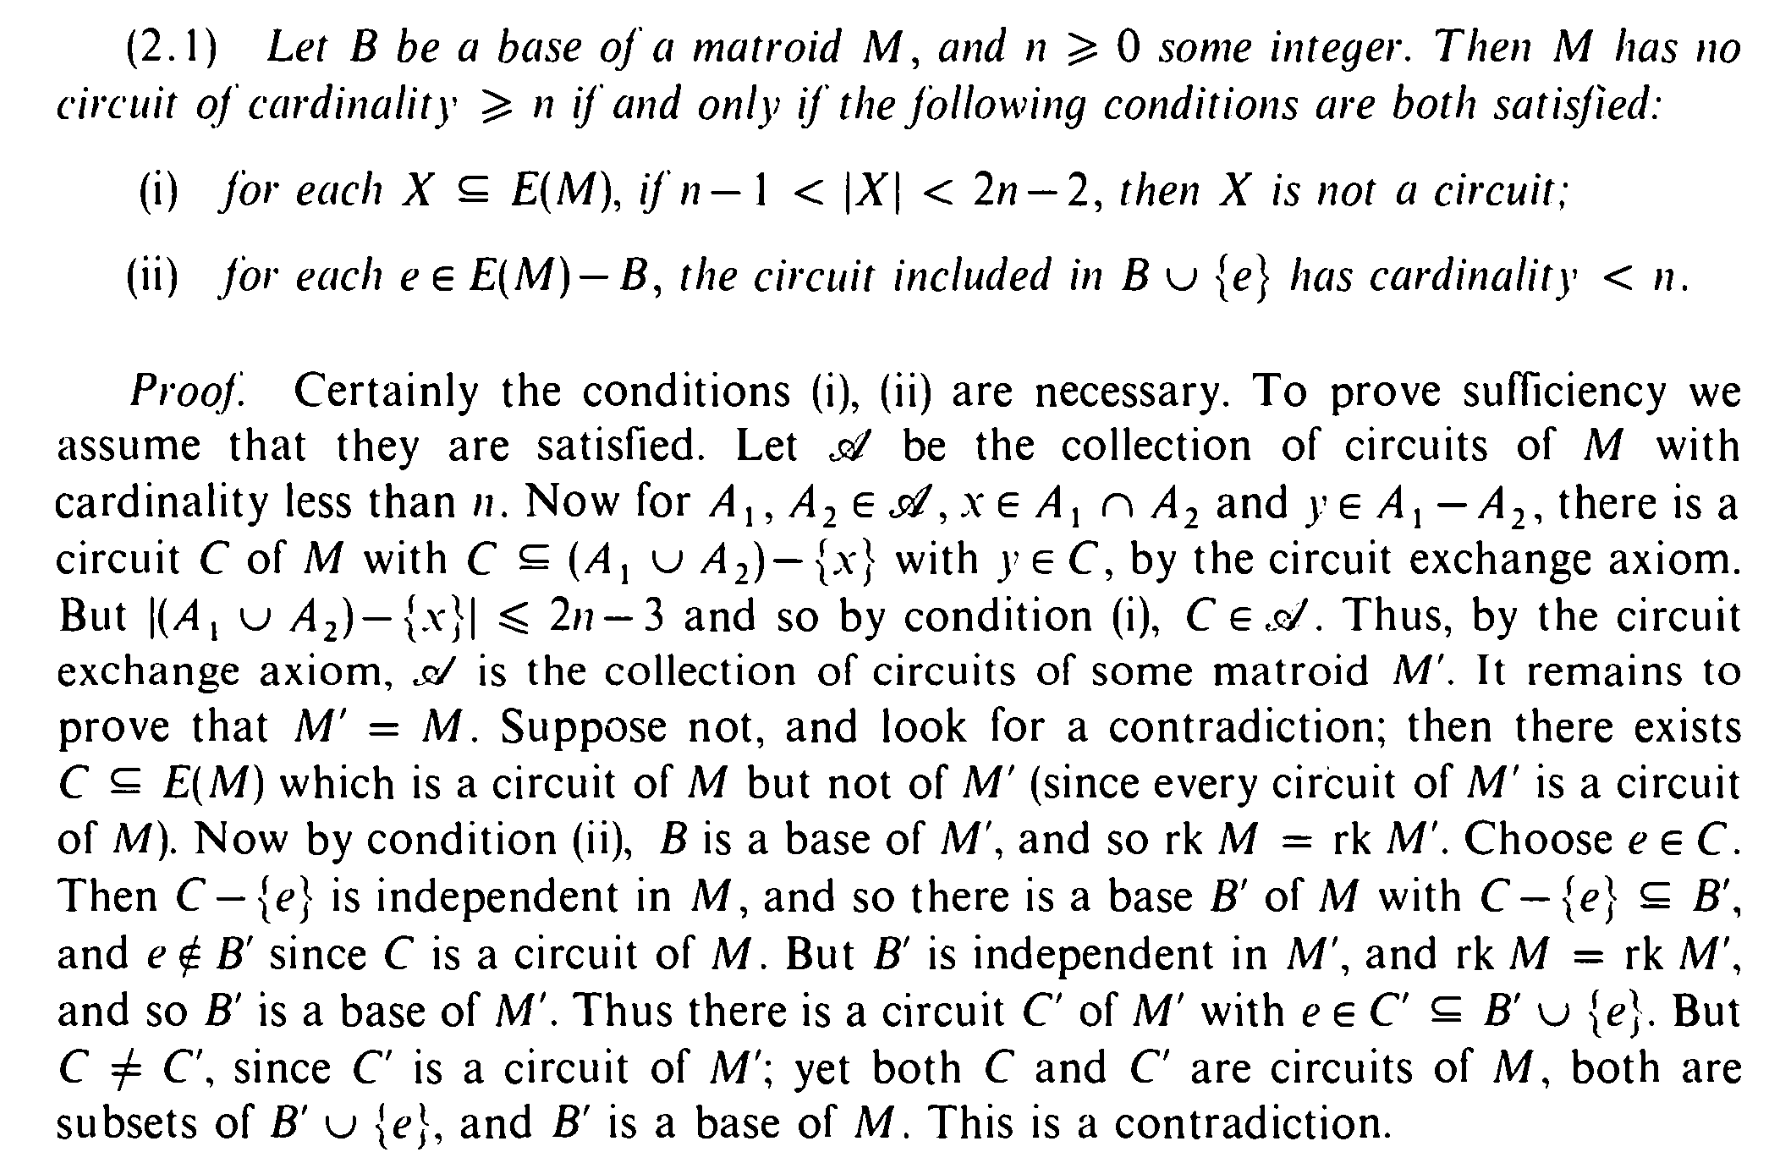
\includegraphics[width=\textwidth]{images/circuitlemma.png}
    \caption{a lemma in \cite{seymour_detecting_1981}}
\end{figure}

\subsection{separable,connected,direct sum...}

\begin{theorem}[theorem 5.2.7]
    $\{S_1,S_2\}$ is a non-empty bi-partition of the ground set $S$. $M=(S,\mathcal{F})$ is the direct sum of $M|S_1$ and $M|S_2$ if and only if $r(S_1)+r(S_2)=r(S)$, where $r$ is the rank function of $M$.
\end{theorem}
\begin{proof}
    If $M$ is indeed the direct sum of $M|S_1$ and $M|S_2$ then $r(S_1)+r(S_2)=r(S)$ by definition.
    If $M$ is not a direct sum and $r(S_1)+r(S_2)=r(S)$. Then there must be a circuit intersecting both $S_1$ and $S_2$. Let this circuit be $C$. $r(C)=|C|-1$ and $r(C\cap S_1)+r(C\cap S_2)=|C|$. $r(S_1)+r(C)\geq r(S_1\cap C)+r(S_1\cup C)$, $r(S_2)+r(C)\geq r(S_2\cap C)+r(S_2\cup C)$, add them up, $r(S_1)+r(S_2)+2|C|-2\geq |C| + r(S_1\cup C)+r(S_2\cup C)$.
    Then we have $r(S_1)+r(S_2)\geq r(S_1\cup C)+r(S_2\cup C)-|C|+2\geq r(S)+|C|-1-|C| +2>r(S)$.
\end{proof}

connected $\equiv$ non-separable $\equiv$ $r(X)+r(S-X)> r(S)$, $X$ is a proper non-empty subset of $S$. 

interesting fact: circuit matroid is connected if and only if the graph is 2-connected.

\mybox{\textbf{Q.} In the proof of theorem 5.2.9, why is CM connected if CB is connected? is it possible that CB is connected but CB' is not connected? 

\textbf{A.}
This problem really confused me. And I think we did not understand the conception of fundamental circuit well. The information can be found at \url{https://proofwiki.org/wiki/Definition:Fundamental_Circuit_(Matroid)}. $B$ is a base of $M=(S,\mathcal{F})$, a fundamental circuit with respect to $B$ means: we choose a element $x \in S - B$, and we can see that $x + B$ is a dependent set. Fundamental circuit is $C \subset x + B$. We can see that $x \in C$ and if we find all fundamental circuits $C_B$ with respect to $B$, $C_B$ has all elements belong to $S - B$ and it also has some elements in $B$. So in hypergraph, $C_B$ is connected, $C_M$ is connected too.}


\subsection{basis}
\begin{theorem}[basis $\leftrightarrow$ independent set]
    $\mathcal B$ satisfies the basis axioms,
    \begin{enumerate}
        \item $\mathcal B$ is not empty
        \item $B_1,B_2\in \mathcal B$, $\forall e\in B_1\setminus B_2$, $\exists f\in B_2\setminus B_1$, s.t. $B_1-e+f\in \mathcal B$
    \end{enumerate}

    $\mathcal F=\{I|\exists B\in \mathcal B, I\subseteq B\}$ satisfies the independent set axioms. The bases of matroid satisfy basis axioms.
\end{theorem}
\begin{proof}
    I1 and I2 holds trivially. We prove the weak independent set exchange property, i.e. $I_1,I_2\in \mathcal F$, $|I_1\setminus I_2|=1$ and $|I_2\setminus I_1|=1$, $\exists e\in I_2\setminus I_2$ such that $I_1+e\in \mathcal F$. 
    First we show that every base has the same size.
    Suppose $B_1,B_2\in \mathcal{B}$ such that $|B_1|\leq |B_2|$ and $|B_1\setminus B_2|$ is minimum. By basis axiom 2 we can find $B_2'=B_2-x+y$, where $x\in B_2\setminus B_1,y\in B_1\setminus B_2$. Consider $B_1$ and $B_2'$, $|B_1|\leq |B_2|=|B_2'|$ and $|B_1\setminus B_2|\geq |B_1\setminus B_2'|$. Thus every base has the same size.
    
    Suppose $I_1$ is contained in a base $B_1$ and $I_2$ is contained in $B_2$. If $B_1=B_2$ then $I_1\cup I_2\in \mathcal F$. Let $\{y\}=B_1\setminus B_2$.
    Thus we assume $B_1\not=B_2$ and $I_2\setminus I_1\not\subseteq B_1$. Now we modify $B_1$ by repeatedly removing elements in $B_1\setminus B_2$(except $y$) from it and adding $B_2\setminus B_1$ to it. Finally $B_2$ contains $y,I_1\cap I_2$ and one element in $I_2\setminus I_1$ at the same time. Thus $I_1$ and $I_2$ satisfy the weak independent set exchange property.

    Bases of matroid(maximal independent set) satisfy basis axioms trivially by the independent set exchange axiom.
\end{proof}

The followings are some basis-exchange properties(see introduction of \cite{Bonin_Savitsky_2016} for references).

\begin{proof}[symmetric basis exchange property]\label{prf:sym_base_exchange}
We need to prove that for two bases $B_1,B_2$ and $x\in B_2$, $\exists y\in B_1\cap C_x$ such that $x\in C_y$. Instead of trying to find such a $y$, we try to find $C_y$ such that $C_y-B_2\subseteq C_x-B_2$ and $x\in C_y$. Note that if such $C_y$ exists, $C_y -B_2$ should contain only one element $y$. So first we further require $|C_y-B_2|$ to be the minimum and try to prove $|C_y-B_2|=1$. Suppose $|C_y-B_2|\not =1$, for any element $z$ in $C_y-B_2$ there is a unique circuit $C_z\subseteq B_2+z$. $C_z$ does not contain $x$ since $|C_z-B_2|<|C_y-B_2|$. Then by strong circuit exchange property we can find a new circuit $C_z'\subseteq C_z\cup C_x-z$ containing $x$. Thus $|C_y-B_2|=1$ and $C_y\subseteq B_2+y$ is the unique circuit of $y$. Since $C_x$ and $C_y$ are both unique, $C_x$ and $C_y$ are the same circuit.
\end{proof}

\begin{theorem}[multiple symmetric exchange property]
    $B_1,B_2\in \mathcal B$, $X\subseteq B_1-B_2$, then there exists $Y\subseteq B_2-B_1$ such that both $B_1-X+Y$ and $B_2+X-Y$ in $\mathcal{B}$.
\end{theorem}
\begin{proof}[\cite{Woodall_1974}]
    The proof is short but not easy. Let $M$ be the original matroid, consider the following matroids,
    \begin{itemize}
        \item $M_1=(M/X)|B_2$($M$ with $X$ contracted, restricted to $B_2$)
        \item $M_2=(M/(B_1-X))|B_2$
        \item $M_3=M_2^*$.
    \end{itemize}
    We need to show that there exists $Y\subseteq B_2$ such that $Y$ is a base of $M_2$ and $B_2-Y$ is a base of $M_1$. In otherwords, $M_1$ and $M_3$ have a common base of size $|B_2-X|$.
    Let $n$ be the rank of $M$. We can easily compute the rank functions for $F\subseteq B_2$,
    \begin{itemize}
        \item $r_1(F)=r(F\cup X)-|X|$
        \item $r_2(F)=r(F\cup( B_1-X))-|B_1-X|=r(F\cup (B_1-X))+|X|-n$
        \item $\begin{aligned}[t]
                r_3(F)&=|F|+r_2(B_2-F)-r_2(B_2)\\
                    &= |F|+ r((B_2-F)\cup(B_1-X))-r(B_2\cup (B_1-X))\\
                    &=|F| + r((B_2-F)\cup(B_1-X))-n
            \end{aligned}$
    \end{itemize}
    Then we want to show that $M_1$ and $M_3$ have a common base of size $|B_2-X|$. Note that the size of maximum common independent set is $\min r_1(F)+r_3(B_2-F)$,
    \begin{align*}
        r_1(F)+r_3(B_2-F) &= r(F\cup X)-|X|+|B_2-F| + r(F\cup(B_1-X))-n\\
                        &\geq r(F\cup X\cup F\cup(B_1-X))+r((F\cup X)\cap (F\cup(B_1-X)))+|B_2-F|-|X|-n\\
                        &= n+r(F)+|B_2-F|-|X|-n\\
                        &=n+|F|+n-|F|-|X|-n\\
                        &=|B_2-X|
    \end{align*}
    Thus max common base of $M_1$ and $M_3$ has size $|B_2-X|$.
\end{proof}
\begin{theorem}[bijective exchange property]
    $B_1,B_2\in \mathcal B$, then there exists a bijection $\sigma: B_1\to B_2$ such that $\forall x\in B_1$, $B_1-x+\sigma(x)\in \mathcal B$.
\end{theorem}
\begin{proof}
    $\sigma(e)=e$ for all $e\in B_1\cap B_2$ so it is enough to find an injection from $B_1-B_2$ to $B_2-B_1$. There exists a unique circuit $C_e\subseteq B_2+e$ for all $e\in B_1-B_2$, so we need to show that the family of $C_e$ satisfies Hall's condition. For $n$ elements $\{e_1,\ldots,e_n\}$ in $B_1-B_2$, $|\bigcup_{i\in[n]}C_{e_i}|\geq n$. Suppose $|\bigcup_{i\in[n]}C_{e_i}|< n$. This is a special case of \autoref{lem:asche}.
    
\end{proof}
\begin{definition}[base-orderable matroid]
    A matroid is base-orderable if for any two bases $B_1,B_2\in \mathcal B$, there exists a bijection $\sigma: B_1\to B_2$ such that for every $e\in B_1-B_2$, both $B_1-e+\sigma(e)$ and $B_2-\sigma(e)+e$ are bases.
\end{definition}

The bijective exchange property holds for any matroid, however not every matroid is base-orderable.

\begin{theorem}[partition basis-exchange property, Theorem 3.3 in \cite{Greene_Magnanti_1975}]
    $B_1,B_2\in \mathcal B$, for each partition $\{P_1,\dots,P_m\}$ of $B_1$ there exists a partition of $B_2=\{Q_1,\dots,Q_m\}$ such that $B_1-P_i+Q_i\in \mathcal B$ for $i\in [m]$.
\end{theorem}

In \cite{Greene_Magnanti_1975} there are proofs of all exchange properties above. These proofs are all generalized from matrix determinant. It seems that extending algebra proofs for linear matroid is a good way to get proofs for general matroids. But I haven't read that paper. Maybe determinant proofs only works for exchange properties.

\begin{proof}[problem 5.3.1]
    By induction. $x_k$ is the only element in $B$ contained in $C_{y_k}$. Thus $B+y_k-x_k\in \mathcal B$. Consider the easier case $B+y_k-x_k$, $x_1,\dots,x_{k-1}$ and $y_1,\dots,y_{k-1}$.
\end{proof}

\begin{proof}[problem 5.3.2]
    We check all the new pairs.
    \begin{itemize}
        \item $t$ and $x\in C(B',t)$. Note that $C(B',t)=C(B,s)$. By (*) $f(s)+1\geq f(x)$ for all $x\in C(B,t)$. Thus $f(t)=f(s)+1\geq f(x)$.
        \item $x\in S-B'$ and $s\in C(B',x)$. We need to prove that $f(s)
        \leq f(x)+1$. Note that the intersection of $C(B',x)$ and $C(B,s)$ is not empty and $t\in C(B,s)$, there exists a circuit containing both $x$ and $t$. Thus $f(s)+1=f(t)\leq f(x)+1$.
    \end{itemize}
\end{proof}

\begin{proof}[problem 5.3.3, circuit and cocircuit never intersect in exactly 1 element]
    $ $
    \newline
    Suppose cocircuit $C^*$ and circuit $C$ intersect in exactly 1 element $e$. Consider the matroid minor $M'=M\backslash(C^*-x)$($M$ with $C^* -x$ deleted). Thus $x$ is a coloop in $M'$ since $C^*$ is the minimal set intersecting every base and $C^*-x$ is deleted. Note that $C$ is still a dependent set in $M'$ since nothing is deleted in $C$. We find a contradiction that circuit $C$ contains a coloop $x$.
\end{proof}
\subsection{generalized partition matroid}

\begin{proof}[problem 5.3.4]
    The only if part is easy. For the if part, one can see that $|F|\leq k$ and $|F\cap S_i|\leq g_i$ for every $i$. Greedily adding elements to $F$ without violating $|F\cap S_i|\leq g_i$ makes a base. Thus $F$ must be a subset of some base and $F$ is independent.
\end{proof}

\begin{definition}[cross-free\cite{schrijver_combinatorial_2003}]
    A family $\mathcal C$ of subsets of a finite set $S$ is called \emph{cross-free} if for all $X, Y \in \mathcal{C}$ one has $X\subseteq Y$ or $Y\subseteq X$ or $X\cap Y=\emptyset$ or $X\cup Y=S$.
\end{definition}
\begin{proof}[problem 5.3.5]
    Suppose $\mathcal{B}$ does not satisfy the basis exchange axiom.
    % Let $B_1,B_2\in \mathcal B$ be a counterexample. $\forall x\in B_1-B_2$, $\nexists y\in B_2-B_1$ s.t. $B_2+x-y\in\mathcal B$. Consider $B_2-y$. We can remove any set containing $y$ in $\{S_1,\dots,S_t\}$ since $|B_2\cap S_i|\leq g_i$. Note that removing every set containing the same elements from a cross-free set system generates a laminar family \cite{schrijver_combinatorial_2003}. 
    Let $B_1,B_2\in \mathcal B$ be a counterexample. $\forall x\in B_1-B_2$, $\nexists y\in B_2-B_1$ s.t. $B_2+x-y\in\mathcal B$. Consider $B_2+x$, there must be a sub-collection $S'=\{S_1,\ldots,S_n\}\subseteq \mathcal{C}$ with $(B_2+x)\cap S_i\leq g_i$ violated. For any two set $S_i,S_j\in S'$ either one contains another or $S_i\cup S_j=S$ since they both contain $x$.
    For any set $S_i$ in $S'$, $S_i$ must contain at least one element in $(B_2-B_1)\cap S_i$ since $|B_1\cap S_i|\leq g_i$. We need to show that $(B_2-B_1)\cap \bigcap_{S_i\in S'} S_i\not=\emptyset$. Suppose the intersection is empty. Note that the minimal set $S_1$ containing $x$ in $S'$ can not be a singleton. Thus there must be some set $S_j\in S'$ such that $S_j=S-S_1+x$. We claim that such $S_j\notin S'$. Note that $|B_1|\leq g_1+g_j-1$ and $|B_2\cap S_1|=g_1$. Thus $|B_2\cap S_j|<g_j$, $S_j\notin S'$. Thus there must exists some element $y$ in $(B_2-B_1)\cap \bigcap_{S_i\in S'} S_i$. Removing $y$ makes $B_2-y+x$ satisfies the constraints.
\end{proof}
\begin{proof}[question 5.3.1]
    I don't know... section 15.3 says $\sum_{S_i} g_i\geq 0$ which is already satisfied.
\end{proof}
\subsection{paving matroid}
Note: $\mathcal H$ is the set of hyperplanes.
\begin{proof}[problem 5.3.6]
    $\BH$ is not empty. If any subset of $S$ of size $r$ is a subset of $H_i$, then the maximal intersection of $H_i$ and $H_j$ will be $r-1$.

    Consider two sets $B_1,B_2\in\BH$. Let $x$ be an element in $B_1-B_2$. We need to prove that $\exists y\in B_2-B_1$ such that $B_1-x+y$ is not a subset of any $H_i$. Note that $B_1-x$ is a subset of at most one $H_i$ since the maximal intersection size is $r-2$. Let $H_1$ be the set which contains $B_1-x$. Suppose there does not exists $y\in B_2-B_1$ such that $B_1-x+y\not\subseteq H_1$. Then $B_2-B_1\subseteq H_1$ and $B_2$ will be a subset of $H_1$. Thus there exists $y\in B_2-B_1-H_1$. $B_1-x+y$ is not a subset of any set in $\mathcal{H}$.
\end{proof}
\begin{proof}[problem 5.3.7]
    The only if part is easy. Every size-$r-1$ subset $I$ of $S$ is the subset of at most one $H_i$ and since $H_i$ is a proper subset of $S$, there is always some base containing $I$. Thus every subset of size $r-1$ or smaller is independent.
    
    The if part. Let $\mathcal{H}$ be the set of hyperplanes of the matroid. $H_i$ is a proper subset of $S$ since there exists elements $e$ in $S-H_i$ such that $H_i+e$ contains a base. $H_i$ has at least $r$ elements since circuits have at least $r$ elements. The intersection of any two set $H_i,H_j\in \mathcal{H}$ has at most $r-2$ elements since otherwise $H_i$ and $H_j$ contains the same rank $r-1$ independent set and they should be the same hyperplane. Thus the set of hyperplanes of the matroid is $\mathcal{H}$ and the matroid is paving.
\end{proof}
\begin{proof}[exercise 5.3.8]
    Already shown in the two proofs above.
\end{proof}

Problem 5.3.7 already showed that an equivalent and simpler way to define paving matroid is through circuit size.

The following is something not in the book. A matroid is called sparse paving if both its dual and itself are paving.

\begin{lemma}
    Any dependent hyperplane in a sparse paving matroid is a circuit.
\end{lemma}
\begin{proof}
    Note that if every hyperplane is independent, then the matroid must be uniform.

    Consider a dependent hyperplane $H$. By its definition we have $r(H)=r-1$ and $|H|\geq r$ where $r$ is the rank of the matroid. Note that the complement of $H$ is circuit in the dual matroid, which is also paving. Thus we have $|H|\geq n-r$. Thus the size of $H$ is exactly $r$. Since dependent sets with size $r$ are circuits, the dependent hyperplane $H$ must be a circuit.
\end{proof}

\subsection{rank}
\begin{proof}
    Suppose R1 R2 and R4 holds. We prove R3 R3' R3'' are equivalent.
    \begin{itemize}
        \item R3' $\to$ R3. By R1 $r(\emptyset)=0$, repeatedly apply R3' from $\emptyset$ to $A$ provides $r(A)\leq |A|$.
        \item R3'' $\to$ R3'. By R4, $r(A\cup e)=r(A\cup e)+r(A\cap e)\leq r(A)+r(e)\leq r(A)+1$ for $e\in S-A$.
        \item R3 $\to$ R3''. R3'' is a special case of R3.($X$ is a singleton)
    \end{itemize}
\end{proof}
\begin{proof}[problem 5.3.10]
    \begin{enumerate}
        \item flats are closed under intersection. Consider two flats $F_1,F_2$ and their intersection $F$. Suppose $F$ is not a flat, i.e. $\exists e\in S-F$ s.t. $r(F)=r(F+e)$. Note that $e$ is contained in at most one of $F_1,F_2$. Assume that $e\in F_1$. Then $r(F_2+e)=r(F_2)$ since $r(F_2)\leq r(F_2+e)$ and $r(F_2+e)+r(F)\leq r(F_2)+r(F+e)$. Thus the intersection $F$ must be a flat.
        \item $H$ is a hyperplane iff $S\setminus H$ is a cocircuit.
        \begin{itemize}
            \item The only if part. Suppose there exists a base $B$ such that $S\setminus H\cap B=\emptyset$. Then $B\subseteq H$ and $r(H)=r>r-1$. $H$ won't be a hyperplane. $S\setminus H$ is the minimal set intersecting every base. If $S\setminus H -x$ still intersects every base for $x\in S\setminus H$, then $r(H+x)=r(H)$ since $H+x$ still does not contain any base.
            \item The if part. $S\setminus H$ intersects every base. Thus $H$ contains no base and $r(H)\leq r-1$. If $r(H)<r-1$ or $H$ is not maximal, there exists at least one element $x\in S-H$ s.t. $H+x$ contains no base. Thus $S-H$ is not minimal.
        \end{itemize}
    \end{enumerate}
\end{proof}
\begin{proof}[problem 5.3.11]\label{proof:5311}
    {\scriptsize $r(S)-r(X)$ implies removing elements in $B-X$}

    Consider the base $B$ with largest intersection with $X$. $I=B\cap X$ is the max independent subset of $X$. Note that $|I|=r(X)$ and $|B\setminus I|=r(S)-r(X)$. $\forall e\in B-I$ there exists a hyperplane $H_e=\cl(B-e)$. Obviously $X\subseteq \bigcap_{e\in B-I}H_e$. Suppose $\exists y\notin X$ but contained in $\bigcap_{e\in B-I}H_e$. One can see that $B+y$ contains a unique circuit $C_y$ and $C_y\cap (B-I)=\emptyset$ since otherwise some $H_e$ won't contain $y$ for $e\in C_y$. Thus $C_y\cap B\subseteq I$ and $y\in X$ since $X$ is a flat.

    If a non-empty set is open then its complement is closed. Then complement of union of cocircuits is the intersection of corresponding hyperplanes by problem 5.3.10. We have proven that every flat is intersection of hyperplanes. Thus the complement of every closed set is the complement of intersection of hyperplanes.
\end{proof}
\begin{proof}[problem 5.3.12]
    see \hyperref[proof:5311]{proof} of problem 5.3.11
\end{proof}
\begin{proof}[problem 5.3.13]
    Obviously the border of a partition of $V$ is the union of edge cuts and edge cuts are cocircuits of the circuit matroid. Already proven in \hyperref[proof:5311]{proof} of problem 5.3.11.
\end{proof}
\subsection{operations on matroids}
\begin{proof}[exercise 5.4.1 adjoint]
    In the new set system $M'=(S+z,\mathcal I')$ let $r'(X)$ be the size of the largest independent set in $X$. For $X\in S$ $r'(X)=r(X)$. Consider $z\in X$. Let $F$ be the largest independent set in $X$. If $z\in F$, $r'(X)=r(X-z)+1$; if $z\notin F$, then $r'(X)=r((X-z)\cup Z)$ since $Z-X$ does not have any contribute to the rank. Now we compare $r(X-z)+1$ and $r(X\cup Z -z)$. One can see that if $z\in F$ $r(X\cup Z -z)\geq r(X-z)+1$ and if $z\notin F$, $r(X-z)+1 \geq r(X\cup Z -z)$. Thus if $z\in X$ the rank function will be $r'(X)=\min\{r(X-z)+1, r(X\cup Z -z)\}$.

    Next we need to show $r'$ is a matroid rank function. Obviously $r'$ satisfies R1,R2,R3 since $r$ is a matroid rank function. We show that $r'$ is submodular.

    ... I think this is very tedious but may not be hard. Showing $\mathcal I'$ satisfies the independent set axioms may be easier. skipped...
\end{proof}

\begin{proof}[exercise 5.4.2 composition]
    Let $B_1,B_2$ be two bases in $\mathcal B$. Let $S_1-F_{11}+F_{21}=B_1$ and $S_1-F_{21}+F_{22}=B_2$ where $F_{11},F_{21}\in \mathcal{I}_1$ and $F_{12},F_{22}\in \mathcal{I}_2$ and $|F_{11}|=|F_{12}|,|F_{21}|=|F_{22}|$. Suppose $|F_{11}|>|F_{21}|$. Since $F_{11}\not=F_{21}$, by independent set exchange property of $M_1$, there exists $x\in F_{11}-F_{21}$ s.t. $F_{21}+x\in \mathcal{I}_1$. Similarly $\exists x'\in F_{12}-F_{22}$ s.t. $F_{22}+x'\in \mathcal{I}_2$. One can see that $B_2-x+x'\in \mathcal{B}$ where $x\in B_2-B_1$ and $x'\in B_1-B_2$. Analysis for $|F_{11}|<|F_{21}|$ and $|F_{11}|=|F_{21}|$ are similar.
\end{proof}
\begin{proof}[exercise 5.4.3]
    Note that $S_1\cap X$ is always independent since $S_1$ is a base. For the rest part $S_2\cap X$, it contains an independent set $F$ if there exists an independent set $F'\subseteq S_1-X$. Thus $r(X)=|S_1\cap X|+\min\{r_2(S_2\cap X),r_1(S_1-X)\}$.
\end{proof}

\textbf{Note}: Theorem 5.4.2 provides an easy way to see union of matroids is a matroid through homomorphic image.

\subsection{dual}
\textbf{Note}: in the proof of theorem 5.4.3 $r^*(X)$ should be the \emph{maximum} size of intersection of a basis of $M$ and $X$... and \emph{maximum} size of intersection of $S-X$ and a basis of $M^*$.

\begin{proof}[exercise 5.4.4]
    I don't want to call $t(X)$ co-rank... every co-thing should be that thing of the dual matroid... $t(X)$ is the minimum size of intersection of $X$ and a base. One can see that when $|X\cap B|$ is minimum $|X\cap B^*|$ is maximum, so $t(X)=|X|-r^*(X)$.
\end{proof}
\begin{proof}[exercise 5.4.5]
    see Theorem 5.2.8 for `connected'.

    If $M$ is connected then by theorem 5.2.8 $r(X)+r(S-X)> r(S)$ for any non-empty proper subset $X$ of $S$. Note that $r(X)=|X|-r^*(S)+r^*(S-X)$. Thus we have $|S-X|+|X|=|S|>|S|-r^*(S)$. The only if part is the same since ${M^*}^*=M$.
\end{proof}
\begin{proof}[exercise 5.4.6]
    Cocircuits are the circuits of the dual matroid. Cocircuit is the minimal set intersecting every base of $M$. Thus by definition none of cocircuits is a subset of a base of the dual matroid(they are dependent in the dual matroid). They are the minimal dependent set since removing any element in a cocircuit $C$ makes $|B\cap C|=0$ for some base $B$. Thus cocircuits are exactly the set of minimal dependent set in the dual matroid.
\end{proof}
\begin{proof}[problem 5.4.7]
    I have read this before.

    Consider the planar dual $G^*$ of some planar graph $G$. We prove that $T\subset E$ is a base if and only if the complement of corresponding edges of $T$ in the planar dual is a base in the dual matroid. Let $T^*$ be the corresponding edges in $G^*$ for $T\subseteq E$. Since ${M^*}^*=M$ and $\overline{\overline{T^*}^*}=T$, we only need to prove one side. Let $T$ be a base of $G$. $\overline{T^*}$ must induce a connected graph in $G^*$ since otherwise $T^*$ contains a cut(cocircuit of $M(G^*)$) and $T$ won't be a base. $\overline{T^*}$ contains no circuit in $G^*$ since otherwise $\overline{T}$ will contain a cut in $G$ and $T$ won't be a base. Thus $\overline{T^*}$ is a base in $G^*$ if $T$ is a base in $G$.
\end{proof}
\subsection{minors}
\begin{proof}[exercise 5.4.8, contraction]
    One can easily see that $r'$ satisfies R1 and R2. For R3, $r'(X)=r(X\cup Z)-r(Z)\leq r(X)+r(Z)-r(X\cup Z)-r(Z)\leq |X|$. For R4, $r'$ is submodular since $r$ is submodular and $(X\cup Z) \cap (Y\cup Z)=(X\cap Y)\cup Z$.
\end{proof}

\begin{proof}[problem 5.4.9]
    Contracting elements in the circuit matroid of a graph corresponds contracting edges in the graph. That is $X\subseteq S-Z$ is independent in $M/Z$ if and only if $X$ is contains no cycle in $G/Z$. By theorem 5.4.4 $X$ is independent in $M/Z$ iff for all maximal independent set $I$ in $Z$, $X\cup I$ is independent in $M$. Note that when contracting edges in $G$ there is a nature injection $\psi$ which maps vertices induced by $Z$ to new vertices $Z'$. Observe that $\forall v\in Z'$ the preimage $\psi^{-1}(v)$ must be connected in $G$. Suppose $X$ contains a cycle in $G/Z$. We claim that $X$ must contain a cycle in $G$. If $X\cup Z'= \emptyset$, then $X$ still contains a cycle in $G$; otherwise $X$ contains a cycle since $\psi^{-1}(x)$ are connected in $G$ for all $x\in X\cup Z'$. Thus if $X$ is independent in $M/Z$, it is independent in the circuit matroid of $G/Z$. The other direction is similar.

    Contracting non-zero vector $z$ in vector matroid is equivalent to projecting the other vectors onto the hyperplane $H_z$ orthogonal to $z$. For any vector $x$, the projected vector is $x-\frac{x\cdot z}{|z|^2}z$. One can easily see that a subset $X$ of the projected vectors is linearly independent if and only if $X\cup z$ is linearly independent.
\end{proof}

\begin{proof}[problem 5.4.10, commutative property]
    We prove that the rank functions are the same.
    $r_{M/Z}(X)=r(X\cup Z)-r(Z)$. $r_{M/Z_1/Z_2}(X)=r_{M/Z_1}(X\cup Z_2)-r_{M/Z_1}(Z_2)=r(X\cup Z)-r(Z)$.

    $r_{(M/Z_2)-Z_1}(X)=r((X-Z_1)\cup Z_2)-r(Z_2)$. $r_{(M-Z_1)/Z_2}(X)=r(X\cup Z_2 -Z_1)-r(Z_2-Z_1)=r_{(M/Z_2)-Z_1}(X)$.
\end{proof}
\begin{proof}[problem 5.4.11, contraction $\equiv$ deletion in the dual matroid]
    $ $
    \newline
    Note that $r^*(X)=|X|-r(S)+r(S-X)$. $r_{M^*-Z}(X)=r^*(X-Z)=|X-Z|-r(S)+r(S-(X-Z))$.

    $r_{(M/Z)^*}(X)=|X|-r_{M/Z}(S-Z)+r_{M/Z}(S-Z-X)=|X|-r(S\cup Z)+r(Z)+r((S-Z-X)\cup Z)-r(Z)=|X|-r(S)+r(S-(X-Z))$. Since $X-Z=X$, $r_{M^*-Z}(X)=r_{(M/Z)^*}(X)$.
\end{proof}

\begin{proof}[problem 5.4.12, minors preserve connectivity]
    $ $
    \newline
    % We have to prove that $r'(X)+r'(S-e-X)> r'(S-e)$ where $X$ is any non-empty proper subset of $S-e$ and $r'$ is the rank function after contracting of deleting $e$ in $M$. Note that if $M$ is connected then $r(e)+r(S-e)> r(S)$. Thus $M$ contains no loop or coloop.
    % \begin{itemize}
    %     \item Deletion. We need to prove $r(X)+r(S-e-X)>r(S-e)$ for any $X\subset S-e$ and $X\not= \emptyset$. Note that $r(S-e)=r(S)$ since $e$ is not a coloop.
    % \end{itemize}
    Matroid dual preserves connectivity.
    % \note{This seems wrong for minors. Consider deleting one element in $U^2_3$(uniform matroid with groundset size 3 and rank 2)}
    For any element $e$, at least one of $M\setminus e$ or $M/e$ is connected if $M$ is connected. See \cite[lemma to theorem II]{crapo_higher_1967}.
\end{proof}
\subsection{matroid connectivity}
\begin{theorem}[prop 5.7 in \href{https://iuuk.mff.cuni.cz/~pangrac/vyuka/matroids/matroid-ch5.pdf}{this notes}]
    A matroid $M$ is connected if
    \begin{enumerate}
        \item $r(X)+r(E-X)>r(E)$ for all non-empty $X\subsetneq E$, or equivalently
        \item for any two elements $x,y\in E$, there is a circuit containing both $x$ and $y$.
    \end{enumerate}
\end{theorem}
\url{https://core.ac.uk/download/pdf/82501331.pdf}

\emph{$k$-separation} of a matroid $M=(E,\mathcal I)$ is a bipartition $\{X,Y\}$ of $E$ such that $\min\{|X|,|Y|\}\geq k$ and $r(X)+r(Y)\leq r(M)+k-1$.

\emph{Vertical $k$-separation} of $M=(E,\mathcal I)$ is a bipartition $\{X,Y\}$ of $E$ such that $\min\{r(X),r(Y)\} \geq k$ and $r(X)+r(Y)\leq r(M)+k-1$.

$M$ is \emph{vertically $n$-connected} if $r(M)\leq n$ and for all $k\in\{1,2,\dots,n-1\}$, $M$ has no vertical $k$-separation.

This is almost the same thing as $n$-vertex connectivity in graphs.


\begin{theorem}
    $M=(E,\mathcal I)$, $n\geq 1$ and $X,Y\subset E$. If $M|X$ and $M|Y$ are both vertically $n$-connected and $r(X)+r(Y)\geq r(X\cup Y)+n-1$, then $M|(X\cup Y)$ is also vertically $n$-connected.
\end{theorem}

(If two $n$ vertex connected graphs have at least $n$ vertices in common, their union is vertex $n$ connected.)



\subsection{matroids from matching}
Given a bipartite graph $G=(S\sqcup T, E)$, \emph{deltoid of base $S$} is defined on $V=S\cup T$. $S$ is a base of the deltoid. For any matching covering $S'\subseteq S$ and $T'\subseteq T$, the symmetric difference of $S$ and $S'\cup T'$ is also a base in the deltoid.
\begin{proof}[deltoid basis axioms]
    Obviously $\mathcal B$ is not empty. We need to show that for two bases $b_1,b_2\in \mathcal B$ and $e\in b_1\setminus b_2$, $b_1-e+f\in \mathcal{B}$ for some $f\in b_2\setminus b_1$. Let $b_1=S-S_1+T_1$ and $b_2=S-S_2+T_2$. Denote the corresponding matchings of $b_1$ and $b_2$ by $M_1$ and $M_2$, respectively. There are two cases,
    \begin{itemize}
        \item $e\in S$. $M_2$ covers $e$ and $M_1$ does not cover $e$. There will be an alternating path $P$, starting from $e$ and containing edges in $M_2$ and $M_1$ alternatively. One can see that the last vertex in $P$ is always in $b_2\setminus b_1$.
        \item $e\in T$. The proof is similar. Find alternating path and the last vertex is $f\in b_2\setminus b_1$.
    \end{itemize}
\end{proof}
\begin{proof}[exercise 5.4.13]
    A matroid is transversal if it is homomorphic image of a partition matroid. Let $M=(S=S_1\sqcup\ldots \sqcup S_n,\mathcal I)$ be the partition matroid and let $\psi$ be the mapping. We construct a new bipartite graph $G=(\psi(S)\sqcup V,E)$. For any part $S_i$ in the partition matroid, we find the set of image $\psi(S_i)$. If $S_i$ has capacity $k$, add $k$ new vertices in $V$ and connect edges between newly added vertices and every vertex in $\psi(S_i)$. One can easily see that a subset of $\psi(S)$ is independent in the homomorphic image of $M$ if and only if it is independent in the transversal matroid of $G$.

    The only if part. The transformation is also easy. Suppose the bipartite graph is $G=(S\sqcup T, E)$ and the transversal matroid is based on $S$. Then for any vertex $u$ in $T$ add $d(u)-1$ copies of $u$ into $T$ and make them a part in the partition with capacity $1$. Again it is not hard to see that a subset of $S$ is independent in the transversal matroid iff it is independent in the homomorphic image of the new partition matroid.
\end{proof}

Again given graph $G=(V,E)$(simple graph but not necessarily bipartite), the \emph{matching matroid} is defined on $V$. A subset of $V$ is independent if it can be covered by some matching. 

Every matching matroid is isomorphic to a transversal matroid.

\subsection{algorithms}
\begin{proof}[problem 5.5.1]
    Just consider elements in decending order of $c_1$ and if there are ties, consider in decending order of $c_2$.

    The proof is identical to the proof of theorem 5.5.2 in the book. For the case $c_1(e)=c_1(f)$, we need to do the argument again for $c_2$.
\end{proof}

I think the author considers max weight base quite differently. For a fix matroid with rank function $r$ and weight function $c:S\to \R$, he defines a vector-rank function $\hat{r}(c):(S\to \R )\to \R$.

\begin{nproblem}[5.5.2]
    Prove that the set of max weight bases satisfies the matroid basis axioms.
\end{nproblem}
\begin{proof}
    Denote the weight function by $w$.

    non-empty. trivial.

    base exchange. Let $b_1,b_2$ be two different bases with the same(maximal) weight. We need to prove that for any element $e\in b_1\setminus b_2$, there exists $f\in b_2\setminus b_1$ such that $b_1-e+f$ is a base of the same maximal weight. There exists a circuit $C_e\in b_2\cup\{e\}$ since $e\notin b_2$. Consider elements in $C_e\cap b_2$. $w(f)\leq w(e)$ for all $f\in C_e\cap b_2$ since otherwise $b_2$ would not be a max weight base. Notice that for any element $e\in b_1\setminus b_2$ the circuit $C_e$ covers $b_2\setminus b_1$. Thus there exists at least one element $f\in C_e\cap b_2$ with $w(f)=w(e)$ since $w(b_1\setminus b_2)=w(b_2\setminus b_1)$. Thus $b_1-e+f$ is still a base with maximal weight.
\end{proof}

\begin{proof}[problem 5.5.3]
    $\underline{\chi}_{Z}$ is the indicator vector of set $Z$. I will write $I_Z$. By theorem 5.5.5, 
    \[
        \hat{r}(c+I_Z)=r(S)c(s_n)+\sum_{i=1}^{n-1} r(S_i)\left( c(s_i)-c(s_{i+1})\right)+r(S)I_Z(s_n)+\sum_{i=1}^{n-1} r(S_i)\left( I_Z(s_i)-I_Z(s_{i+1})\right)
    \]
    One can see that $I_Z(s_i)$ contributes to the sum by 1 if and only if $r(S_i)=r(S_{i-1})+1$. Thus $\hat{r}(c+I_Z)=\hat r(c)+r_c(Z)$.

\end{proof}

Proofs of problem 5.5.4-5.5.6 are easy

\begin{nproblem}[5.5.7]
    determine algorithmically if an independent set $I$ can be extended to a max weight base.
\end{nproblem}
For this problem, consider elements in $S-I$ in decending order of weights. Select the current element if it is independent from the set of previously selected elements and $I$. (contract $I$ in the matroid)

Actually all different max weight bases can be generated through the greedy algorithm with different tie breaking rules. Suppose there is a max weight base $B'$ which can not be generated by the greedy algorithm. Consider the set of max weight bases generated by the greedy algorithm by any tie breaking rules. Let $B$ be the base with largest intersection with $B'$. Let $f$ be the elements with largest weight in $B-B'$. By the base exchange property, there exists a element $e\in B'-B$ such that swapping $e$ and $f$ still generates bases. We know that $w(f)=w(e)$. Then for some tie breaking rules the greedy algorithm will add $e$ to the base instead of $f$, which contradicts the assumption that $B'$ can not be generated by any tie breaking rules.

\begin{nproblem}[5.5.8]
    determine algorithmically if there is a base which is simultaneously maximal with weights $w_1,\dots,w_k$.
\end{nproblem}
Sort elements lexicographically based on the vector $w(e)=(w_1(e),\dots,w_k(e))$ and use the greedy algorithm to find a max weight base $B^*$. Then check whether $B^*$ is the simultaneously maximal with weights $w_1,\dots,w_k$.
\begin{proof}
    We need to prove that if there exists a common max base for weights $w_1,\dots,w_k$, then the lexicographically max base is simultaneously maximal with weights $w_1,\dots,w_k$. 
    Let $B$ be the base computed by the lexicographically sorted greedy algorithm.
    Suppose $B$ is not a common max base for weights $w_1,\dots,w_{k}$. Then we can find a common max base $B'$ which has intersection with $B$ as large as possible. Let $f$ be the (lexicographically) largest element in $B\setminus B'$. By the matroid base exchange property there exists $e\in B'\setminus B$ such that $B-f+e$ and $B'+f-e$ are bases.

    If $e$ is lexicographically smaller than $f$(denoted by $e\prec f$), then $B'-e+f$ will be a larger base than $B'$ for some weight. If $e\succ f$, then the greedy algorithm will add $e$ to the base before $f$ and such $B$ can not exist. If $e=f$, then $B'+f-e$ is a common max base and has larger intersection with $B$. Thus such $B'=B$. The greedy algorithm finds the common max base if one exists.
    \scriptsize{when dealing with the greedy base algorithm, proofs always look like this.}
\end{proof}

\begin{proof}[problem 5.5.9]
    We prove this by induction on $k$. $k=1$ is trivial. Suppose the statement is true for all $k\leq p$. Consider the $k=p+1$ case. Notice that $B'=B-x_{p+1}+y_{p+1}$ is a base with the same weight as $B$. We claim that the conditions in the statement still holds for $B'$.
    (That is, $y_1,\dots,y_{p}$ and $x_1,\dots,x_{p}$ satisfy that $c(x_i)=c(y_i)$ and $x_i\in C(y_i,B')$. Furthermore, $h>j$ and $c(x_h)=c(y_j)$ imply that $x_h \notin C(y_j,B')$.)
    Now consider the circuits $C(y_i,B)$ for $i\in [p]$, if $C(y_i,B)$ doesn't contain $x_{p+1}$, the conditions obviously holds. Now suppose that $C(y_i,B)$ contains $x_{p+1}$, we know that there exists a circuit $C$ such that  $y_i\in C\subseteq C(y_1,B)\cup C(y_i,B)\setminus \{x_{p+1}\}$. $C$ also contains $y_{p+1}$ since otherwise $C(y_i,B)$ is not unique. Note that $c(y_i)>c(y_{p+1})$ since $h>j$ and $c(x_h)=c(y_j)$ imply that $x_h \notin C(y_j,B')$ and we have already assumed $x_{p+1}\in C(y_i,B)$.
    We can see that $B'$ is not a max weight base since we can swap $y_{p+1}$ and $y_i$ to increase the weight. Thus $x_{p+1}\notin C(y_i,B')$. All conditions holds for $B'$.
\end{proof}

\subsection{polyhedron}

Consider the following LPs,

\begin{minipage}{.45\textwidth}
\begin{align*}
    \text{LP1: } \max  cx\\
    s.t. \quad x(Z)&\leq r(Z) &\forall Z \subsetneq S\\
                x(S)&=r(S) \\
                x&\geq 0
\end{align*}
\end{minipage}
\begin{minipage}{.45\textwidth}
\begin{align*}
    \text{Dual1: } \min \sum_{Z\subseteq S} y_Z r(Z)\\
    s.t. \quad \sum_{s\in Z}y_Z&\geq c(s) & \forall s\in S\\
    y_Z&\geq 0 & \forall Z\subsetneq S
\end{align*}
\end{minipage}

\begin{minipage}{.45\textwidth}
\begin{align*}
    \text{LP2: } \max  cx\\
    s.t. \quad x(Z)&\leq r(Z) &\forall Z \subseteq S\\
                x&\geq 0
\end{align*}
\end{minipage}
\begin{minipage}{.45\textwidth}
    \begin{align*}
        \text{Dual2: } \min \sum_{Z\subseteq S} y_Z r(Z)\\
        s.t. \quad \sum_{s\in Z}y_Z&\geq c(s) & \forall s\in S\\
        y_Z&\geq 0 & \forall Z\subseteq S
    \end{align*}
\end{minipage}

LP1 and LP2 are both total dual integral.

Define the independence polytope $P(M)=\conv\{\underline{\chi}_I, \forall I\subseteq \mathcal I(M)\}$ and the base polytope $B(M)=\conv\{\underline{\chi}_B, \forall B\subseteq \mathcal B(M)\}$.

\begin{theorem}[5.5.8]
    Let $B'$ and $P'$ be the polyhedrons described in LP1 and LP2 respectively. Then $B'=B(M)$ and $P'=P(M)$.
\end{theorem}
\begin{proof}
    Clearly $B(M)\subseteq B'$ and $P(M)\subseteq P'$. Now we show that $B'\subseteq B(M)$ and $P'\subseteq P(M)$. We know that LP1 and LP2 are TDI and all numbers in the LPs are integer. Thus all extreme points of $B'$ and $P'$ are integer. By definition one can see that the extreme points of $B'$ and $P'$ are exactly the indicator vectors of bases and independent sets since otherwise they won't satisfy the rank function inequalities. Thus $B'\subseteq B(M)$ and $P'\subseteq P(M)$.
\end{proof}

A set function $f$ is a polymatroid function if $f(\emptyset)=0$, $f$ is non-decreasing and $f$ is submodular. If $f$ is also subcardinal, then $f$ will be a matroid rank function.

\begin{proof}[problem 5.5.10]
    $\gamma(X)=|\Gamma_G(X)|$ for $X\subseteq S$ is a polymatroid function.(The number of vertices in $T$ which connected with $X$.) $\gamma(\emptyset)=0$ and non-decreasing properties are easy to verify. $\gamma(X)$ is submodular since $\gamma(X)+\gamma(Y)=|\Gamma_G(X)|+|\Gamma_G(Y)|=|\Gamma_G(X)\cup \Gamma_G(Y)|+|\Gamma_G(X)\cap\Gamma_G(Y)|\geq |\Gamma_G(X\cup Y)|+|\Gamma_G(X\cap Y)|$.

    An integral vector $m\in \Z_+^S$ belongs to the polymatroid set determined by $\gamma$ iff $\exists F\subseteq E$ s.t. $d_F(t)\leq 1$ for every $t\in T$ and $d_F(s)=m(s)$ for every $s\in S$. 
    The only if part. $m\in \Z_+^S$ is an integral vector such that $\widetilde{m}(X)\leq |\Gamma_G(X)|$ for all $X\subseteq S$. We claim that it is always possible to select $F\subseteq E$ as the edges achieving $\Gamma_F(s)=m(s)$ and keeping $d_F(t)\leq 1$ for every $t\in T,s\in S$. Suppose that $\Gamma_F(s)=m(s)$ for every $s\in S$ but $d_F(t)> 1$ for some $t\in T$. There will be $s_1,s_2$ such that there exists edges $(s_1,t),(s_2,t)\in F$. We also have $m(s_i)=d_F(s_i)=|\Gamma_G(s_i)|$ since otherwise we can simply swap one of the edges$(s_i,t)$ with $(s_i,z)\notin F$. However in this case $m(\{s_1,s_2\})>|\Gamma_G(\{s_1,s_2\})|$. Thus we can always find the desired $F\subseteq E$.
    The if part is easy. $m(X)\leq |\Gamma_G(X)|$ since $d_F(t)\leq 1$ for all $t\in T$.
\end{proof}

\begin{proof}[exercise 5.5.11]
    One can easily see that $e_H(\emptyset)=0$ and $e_H(X)$ is non-decreasing.
$e_H(X)+e_H(Y)=e_H(X\cup Y)+e_H(X\cap Y)+\text{\# hyperedges intersecting both $X\setminus Y$ and $Y\setminus X$} \geq e_H(X\cup Y)+e_H(X\cap Y)$.
\end{proof}

\mybox{
    \begin{theorem}[Orientation lemma, theorem 2.3.2 in the book]\label{lem:orient}
    For undirected graph $G=(V,E)$, and a function $m:V\to \Z$ satisfying $\widetilde{m}(V)=|E|$, the followings are equivalent. Let $\rho(v)$ be the in-degree of $v\in V$, $i_G(X)$ be the number of edges induced by $X$ in $G$ and $e_G(X)$ be the number of edges with at least one end-point in $X$.
    \begin{enumerate}
        \item $G$ has an orientation so that $\rho(v)=m(v)$ for every node $v$,
        \item $e_G(X)\geq \widetilde{m}(X)$ for every subset $X\subseteq V$,
        \item $i_G(Y)\leq \widetilde{m}(Y)$ for every subset $Y\subseteq V$.
    \end{enumerate}
    \end{theorem}
}
\begin{proof}[problem 5.5.12]
    By \autoref{lem:orient} we have $m\leq e_G$. $\widetilde{m}(V)=e_G(V)$ since the sum of in-degree is exactly the number of edges. Thus $Z_{in}$ is the set of integral elements of the base-polyhedron.
\end{proof}
\paragraph{Polymatroid greedy algorithm} Consider the following LPs,

\begin{minipage}{.45\textwidth}
\begin{align*}
    \text{LP3: } \max  cx\\
    s.t. \quad x(Z)&\leq f(Z) &\forall Z \subseteq S\\
                x&\geq 0
\end{align*}
\end{minipage}
\begin{minipage}{.45\textwidth}
    \begin{align*}
        \text{Dual3: } \min \sum_{Z\subseteq S} y_Z f(Z)\\
        s.t. \quad \sum_{s\in Z}y_Z&\geq c(s) & \forall s\in S\\
        y_Z&\geq 0 & \forall Z\subseteq S
    \end{align*}
\end{minipage}

This looks almost the same as LP2 and Dual2, but here $f$ is a polymatroid function instead of a matroid rank function. Why does the greedy algorithm works on matroids?

\begin{enumerate}
    \item We can discard all elements with negative weights. If any set $Z\subseteq S$ satisfies $x(Z)\leq r(Z)$, so does any subset of $Z$. This also works if $r$ is a polymatroid function.
    \item Suppose no further information than 1. is provided, what we can do is enumerating all subsets and finding the one with the largest weight. So why does greedy alg work? I think it is because the independent set exchange property. In LP2 $x(s)$ is automatically in $[0,1]$. Thus $x$ is naturally the indicator vector of subsets of $S$. For two independent sets $A,B$ with $|A|=|B|$, if there exists an element $a\in A\setminus B$ such that $c(a)$ is larger than the weight of any element in $B\setminus A$, we can always apply the independent set exchange property to make $c(B)$ larger. Thus it is always valid to select the largest element(if it doesn't break independence).
\end{enumerate}

However 2. for polymatroid functions (see LP3) is more complicated. In LP3 $x$ is no longer indicator vector of subsets of $S$ since $f$ is not subcardinal. Now it is reasonable to write $x_{alg}$ as (5.27) and to proof lemma 5.5.10 and theorem 5.5.11.

\subsection{matroids vs polymatroids}
Theorem 5.5.14 is important and the proof is tricky. I think it's worth a careful reading.
\begin{proof}[exercise 5.5.13]
    It follows from the definition of $b_r$ and the monotonicity of $r$ that $b_r(\emptyset)=0$ and $b_r$ is non-decreasing. For any $A\subseteq B\subseteq S$ and $e\in S\setminus B$, one can see that $\psi^-(e)$ has empty intersection with $\psi^-(A)$ and $\psi^-(B)$. Thus by submodularity of $r$ we know that $b_r(B+e)-b_r(B)=r(\psi^-(B)\cup \psi^-(e))-r(\psi^-(B))\leq r(\psi^-(A)\cup \psi^-(e))-r(\psi^-(A))=b_r(A+e)-b_r(A)$.
\end{proof}

\begin{proof}[exercise 5.5.14]
    I can't find a mapping directly. However if using theorem 5.5.16 is allowed, we only need to show that $e_G$ is polymatroidal. There is a construction in the proof of theorem 5.5.16.
\end{proof}

\begin{proof}[problem 5.5.15]
    It follows from theorem 5.5.17 that we only need to prove that the edges of $G'$ is independent set of a matroid. Suppose there are two subgraphs $G_1=(V,F)$ and $G_2=(V,H)$ both satisfying the condition that $d_{G_i}(v)\leq g(v)$ for all $v\in V$. We prove the weak independent set exchange property. Assume that $|F\setminus H|=2$ and $|H\setminus F|=1$. Suppose $F$ and $H$ violate the exchange property. Let $h=H\setminus F$. $F+h$ does not satisfy the condition since otherwise $F\cup H$ is independent. Thus there exists a 'circuit'(It is not a matroid yet) $C\subset F+h$. $C\cap (F\setminus H)$ is not empty since otherwise $F$ is not independent. Consider the induced graph of $F\cup H$. Removing any edge in $C$ will make the whole graph independent. Thus one of the two edges in $F\setminus H$ can be added to $H$ while keeping independence. Thus edges of $G'$ indeed form the independent set of a matroid. The rest of the proof is just applying theorem 5.5.17.
\end{proof}